%!TEX root = origin_elements_lecture_notes.tex

\chapter{Star Formation}\label{sec:star_formation}

In the last chapter we discussed the formation of the first elements in the Big Bang and derived that all the hydrogen and the vast majority of helium we see today in the universe formed in this event. In this chapter we will study how stars can form from hydrogen and helium gas and how they evolve throughout their lifetime. This topic is discussed generally for all stars, however, we will in the end focus on the very first and oldest star to form in the galaxy.

\section{Molecular Cloud Collapse and Protostar Formation}

\begin{figure}[tb]
    \centering
    \begin{subfigure}{0.44\textwidth}
        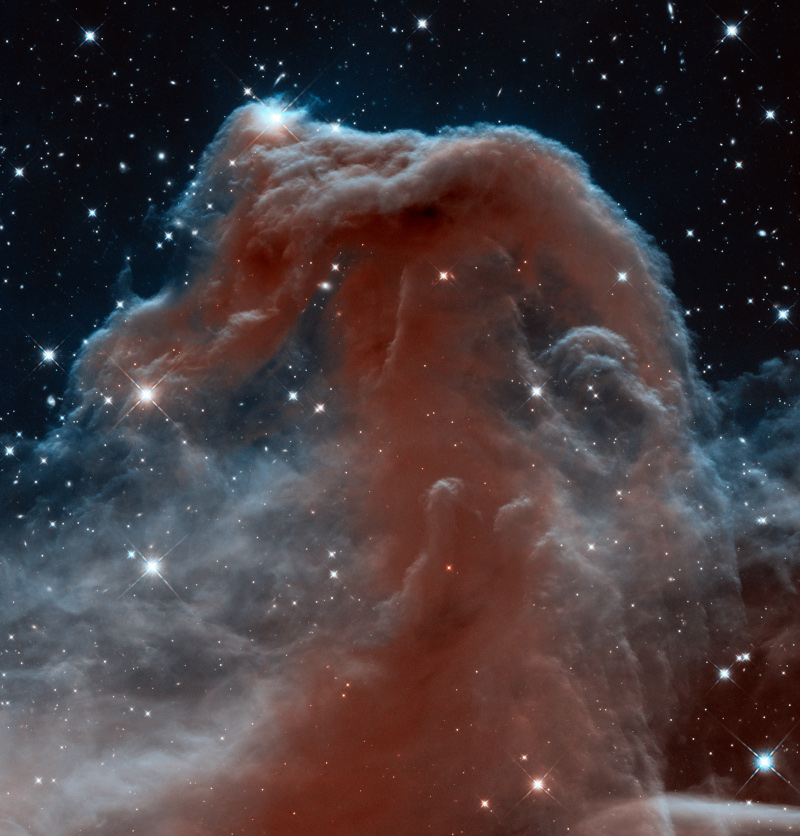
\includegraphics[width=\textwidth]{graphics/star_formation/horsehead_nebula}
        \caption{The horsehead nebula. Credit: NASA/ESA/Hubble Heritage Team.}
        \label{fig:star_formation:horsehead_nebula}
    \end{subfigure} \qquad
    \begin{subfigure}{0.459\textwidth}
        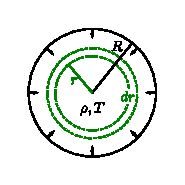
\includegraphics[width=\textwidth]{graphics/star_formation/molecular_cloud_collapse.pdf}
        \caption{A schematic representation of a molecular cloud collapsing.}
        \label{fig:star_formation:cloud_collapse_schematic}
    \end{subfigure}
    \caption{Molecular clouds are the structures stars form from in the universe.}
    \label{fig:star_formation:molecular_clouds}
\end{figure}
To understand star formation, let us first discuss how molecular clouds collapse. Figure~\ref{fig:star_formation:horsehead_nebula} shows a \ac{hst} image of the famous horsehead nebula, a molecular cloud located in the constellation Orion. Molecular clouds are accumulations of gas and dust in the galaxy that prevent light from the stars behind it to come through. These structures thus look like clouds to the observer.

\subsection{Jeans Criterium for Gravitational Collapse}

For simplicity, let us assume a spherical, homogeneous sphere with a constant density $\rho$ and temperature $T$. A schematic of such an idealized molecular cloud is shown in Figure~\ref{fig:star_formation:cloud_collapse_schematic}. The gravitational / potential that a given test mass $m$ in the molecular cloud is in can be written as
\begin{equation}
    E_\mathrm{pot} = -\frac{GMm}{R}.\label{eqn:star_formation:potential_energy}
\end{equation}
Here, $R$ is the distance of the test mass from the center of the molecular cloud and $M$ is the total mass of the cloud inside the radius $R$. Furthermore, $G$ is the gravitational constant and is equal to $G=6.674 \times 10^{-11}$\,m$^{3}$\,kg$^{-1}$\,s$^{-2}$. Infinitely far away from the molecular cloud, the gravitational potential is by definition zero. Thus, it becomes negative the closer to the center the test mass gets. 

Instead of a test mass, let us now assume that we want to determine the gravitational energy of a mass shell with thickness $dr$ at distance $r$ from the center of the molecular cloud. A schematic of this setup is shown in Figure~\ref{fig:star_formation:cloud_collapse_schematic}. Assuming that the cloud is at a given temperature $T$ and has a homogeneous density $\rho$, we can write the mass of the shell ($m$) and the mass of the cloud inside the shell ($M$) as
\begin{eqnarray}
    m &=& 4 \pi \rho r^2 dr \label{eqn:star_formation:mass_molecular_cloud_shell} \\
    M &=& \frac{4}{3} \pi \rho r^3 \label{eqn:star_formation:mass_molecular_cloud}.
\end{eqnarray}
We can now determine the total potential energy of the molecular cloud as
\begin{equation}
    \begin{aligned}
        E_\mathrm{pot} &= -\int_0^R \frac{G}{r}\left( \frac{4}{3} \pi \rho r^3\right) \left( 4\pi \rho r^2\right) dr \\
        &=  -\frac{16}{3} \pi^2 \rho^{2} G \int_0^R r^4 dr \\
        &= -\frac{16}{15} \pi^2 \rho^2 GR^5 \\
        &= -\frac{3}{5}G\frac{M^2}{R}.
    \end{aligned}
    \label{eqn:star_formation:epot}
\end{equation}
In the last step we used the fact that the mass of the molecular cloud can be written as
\begin{equation}
    M = \frac{4}{3} R^3 \rho
\end{equation}
to substitute it back into the equation.

During the collapse, gravitational energy is transformed into kinetic energy, which here is equal to a rise in temperature. The total kinetic energy of the system can be written as
\begin{equation}
    E_\mathrm{kin} = \frac{3}{2} NkT = \frac{3}{2} kT \frac{M}{\mu}, \label{eqn:star_formation:ekin}
\end{equation}
where $N$ is the number of molecules in the molecular cloud and $\mu$ their average mass, i.e., to first approximation the mass of H$_2$.
For a cloud in hydrostatic equilibrium, i.e., a cloud that is neither expanding nor contracting, the virial theorem (which is derived in Appendix~\ref{app:virial_theorem}) can be applied. This theorem states that the kinetic and potential / gravitational energy are related to each other as
\begin{equation}
    2 E_\mathrm{kin} + E_\mathrm{pot} = 0. \label{eqn:star_formation:virial_theorem}
\end{equation}
Assuming the molecular cloud is in equilibrium, we can plug equations~\eqref{eqn:star_formation:epot} and~\eqref{eqn:star_formation:ekin} into~\eqref{eqn:star_formation:virial_theorem} and solve for the mass.
\begin{equation}
    \begin{aligned}
        3 kT \frac{M}{\mu} - \frac{3}{5}G \frac{M^2}{R} &= 0\\
        \frac{GM}{5R} &= \frac{kT}{\mu}\\
        M &= \frac{5RkT}{G\mu} \equiv M_J
    \end{aligned}\label{eqn:star_formation:jeans_mass_derivation}
\end{equation}
Here, $M_J$ is the so-called Jeans mass, named after Sir James Jeans who first described this derivation in 1904. It describes the mass $M=M_J$ for which the molecular cloud is in balance, i.e., the kinetic and gravitational energy compensate each other. The Jeans mass thus also describes the minimum mass for star formation; a molecular cloud with $M>M_J$ will collapse since the gravitational force dominates.


\subsection{Free Fall Time}

To determine how long gravitational collapse of a molecular cloud takes, we can estimate the free fall time. The gravitational force of the system and its radius are known. Using Newton's law $\vec{F} = m\vec{a}$, we can thus write the slightly unwieldy differential equation
\begin{equation}
    -G\frac{Mm}{R^2} = m\ddot{R},
\end{equation}
where $m$ is a test mass at the edge of the cloud. However, the free fall time $\tau_\mathrm{ff}$ can also be derived more elegantly. Kepler's third law of planetary motion states that the cube of the semi-major axis of a planet divided by the square of its period is constant. This law in fact can directly be derived by comparing the gravitational and centrifugal force acting on a planet since these two forces, for a stable orbit, must compensate each other.
\begin{figure}[tb]
    \centering
    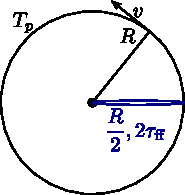
\includegraphics[width=0.3\textwidth]{graphics/star_formation/kepler3}
    \caption{Schematic to derive the free fall time $\tau_\mathrm{ff}$ using Kepler's third law of planetary motions. See text for details.}
    \label{fig:star_formation:kepler3_free_fall_time_schematic}
\end{figure}
Figure~\ref{fig:star_formation:kepler3_free_fall_time_schematic} shows a schematic of the here discussed scenario. The molecular cloud (black circle), if not collapsing, would have to rotate at a given velocity $v$ such that the gravitational force $F_\mathrm{g}$ and the centrifugal force $F_\mathrm{c}$ compensate each other. For a test mass at the outermost edge of the cloud, the gravitational force of the whole cloud is equivalent as if we pictured the mass of the cloud to be concentrated in the center. Disregarding vector quantities, we can derive the velocity a stable cloud would move around the center with as
\begin{equation}
    \begin{aligned}
        F_\mathrm{g} &= F_\mathrm{c} \\ 
        G\frac{Mm}{R^2} &= \frac{mv^2}{R}\\
        \Rightarrow v &= \left(G\frac{M}{R}\right)^{\nicefrac{1}{2}}.
    \end{aligned}
    \label{eqn:star_formation:velocity_orbit_stable_molecular_cloud}
\end{equation}
k
To determine the free fall scenario we can now halt the test particle in its motion, i.e., set $v=0$. The ``orbit'' of the test particle would then look like a straight line into the gravitational center of the cloud. In Figure~\ref{fig:star_formation:kepler3_free_fall_time_schematic} this scenario is shown by drawing the line as a very skinny ellipse. The semi-major axis of this orbit would now be $R/2$ and the orbital period $2\tau_\mathrm{ff}$. 

From Kepler's third law we know that the following statement must hold true.
\begin{equation}
    \frac{R^{3}}{T_P^2} = \frac{\left(\frac{R}{2}\right)^{3}}{(2\tau_\mathrm{ff})^2}
    \label{eqn:star_formation:kepler3_free_fall_time}
\end{equation}
Here, $T_P$ can be derived using the velocity as given in equation~\ref{eqn:star_formation:velocity_orbit_stable_molecular_cloud} and the length of the orbit ($2\pi R$). This yields
\begin{equation}
    T_p = 2\pi \left(\frac{R^{3}}{GM}\right)^{\nicefrac{1}{2}}.
    \label{eqn:star_formation:period_orbit_stable_molecular_cloud}
\end{equation}
Plugging equation~\eqref{eqn:star_formation:period_orbit_stable_molecular_cloud} into equation~\eqref{eqn:star_formation:kepler3_free_fall_time} and expressing the mass of the cloud using the density $\rho$ as $M=\frac{4}{3}R^3\rho \pi$, we can finally derive the free fall time as
\begin{equation}
    \tau_\mathrm{ff} = \left( \frac{3\pi}{32G\rho}\right)^{\nicefrac{1}{2}}.
\end{equation}


\subsection{Protostar Birth}

Fortunately, the molecular cloud collapse does not take place adiabatically. Heat is effectively radiated from the cloud as \ac{ir}, thus preventing the Jeans mass (which is proportional to the temperature) from exceeding the molecular cloud mass and thus bringing the cloud into hydrostatic equilibrium (see Section~\ref{sec:star_formation:hydrostatic_equilibrium}). The main cooling mechanisms producing \ac{ir} radiation are molecular collisions and dust. Colliding molecules transfer energy into vibrational states which, when they decay, emit \ac{ir}. Dust on the other hand will heat up and radiate as a blackbody with an effective temperature of less than around 1000\,K, thus mostly radiating in the \ac{ir}. The molecular cloud is mostly transparent to \ac{ir} and can thus effectively cool thanks to these processes.

Ultimately, the rising heat will start dissociating molecules and evaporating dust, thus the effective cooling mechanism stops. At this point the temperature in the center rises and the Jeans mass will be exceeded. The center of the collapsing cloud defines the protostar in hydrostatic equilibrium (see below).



\section{Hydrostatic equilibrium} \label{sec:star_formation:hydrostatic_equilibrium}

Once a molecular cloud has reached a high enough temperature such that its mass is equal to the Jeans mass, the system has entered the so-called hydrostatic equilibrium. Understanding this equilibrium is crucial in terms of understanding stellar phases during the end of their lives and during nucleosynthesis events. The whole life of a star is dominated by hydrostatic equilibrium. 

\begin{figure}[tb]
    \centering
    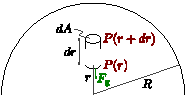
\includegraphics[width=0.4\textwidth]{graphics/star_formation/hydrostatic_equilibrium}
    \caption{Schematic drawing to derive the hydrostatic equilibrium equation. See text for details.}
    \label{fig:star_formation:hydrostatic_equilibrium_schematic}
\end{figure}
Figure~\ref{fig:star_formation:hydrostatic_equilibrium_schematic} shows a cylinder of length $dr$, face area $dA$, and density $\rho(r)$ at distance $r$ from the center of the star. The gravitational force that acts on the cylinder can be written as
\begin{equation}
    F_\mathrm{g} = -G\frac{M_r dm}{r^2},
    \label{eqn:star_formation:hydrostatic_equilibrium_gravitational_force}
\end{equation}
where $M_r$ is the mass of the star that is inside radius $r$ and $dm = \rho(r) dr dA$ is the mass of the cylinder. 


In addition, the cylinder is under pressure, i.e., the pressure $P(r+dr)$ from above it pushing it down and the pressure $P(r)$ from below it pushing it up. To force exerted by the pressure is 
\begin{equation}
    F_P = dPdA,
    \label{eqn:star_formation:hydrostatic_equilibrium_pressure_force}
\end{equation}
where $dP = P(r+dr) - P(r)$.

In order for the cylinder to be neutrally buoyant, i.e., to be in hydrostatic equilibrium, the gravitational force must exactly compensate the force exerted by the pressure. Setting equations~\eqref{eqn:star_formation:hydrostatic_equilibrium_gravitational_force} and~\eqref{eqn:star_formation:hydrostatic_equilibrium_pressure_force} equal plus some simple algebra, we can derive the hydrostatic equilibrium condition as
\begin{equation}
    \frac{dP}{dr} = -\rho(r) \frac{GM_r}{r^2}.
    \label{eqn:star_formation:hydrostatic_equilibrium}
\end{equation}

\subsection{Central Pressure}

Using equation~\eqref{eqn:star_formation:hydrostatic_equilibrium}, we can estimate the central pressure of a star by integrating over $r$. For this estimate, let us replace the density $\rho(r)$ with the mean density inside the star. This mean density can be expressed as
\begin{equation}
    \bar{\rho} = \frac{M}{\frac{4}{3} \pi R^3}.
\end{equation}
We can furthermore write $M_r$ as a function of the distance $r$ from the center of the star. Remember that $M_r$ simply represents the mass of the star inside of radius $r$, thus
\begin{equation}
    M_r = M(r) = \frac{4}{3} \pi r^3 \bar{\rho}.
\end{equation}
Plugging these two quantities into equation~\eqref{eqn:star_formation:hydrostatic_equilibrium} and integrating over $r$, the central pressure $P_c$ can be estimated as
\begin{equation}
    P_c = \frac{3}{8\pi}\frac{GM^{2}}{R^{4}}.
    \label{eqn:star_formation:central_pressure}
\end{equation}
We assumed here that the pressure at the surface of the star is zero, which is surely true when compared to the central pressure. In the case of the Sun, using equation~\eqref{eqn:star_formation:central_pressure} we can calculate a central pressure of $P_{c,\odot} \approx 10^{14}$\,Pa.

Note that the presented estimate of the central pressure of a star necessarily represents a lower limit. The reason for this is that we assumed a constant density throughout the star, which surely is not correct. The density will be significantly higher in the center of the star compared to the outer parts. This always increases the pressure compared to our estimate. To visualize why, imagine all the mass of the star was concentration within $R/2$. Integrating the pressure over the whole star using our estimate above would result in the same central pressure. However, from our visualization we know that the central pressure is concentrated in the inner half, thus integration of $r$ only needs to be done up to $R/2$ to determine the ``real'' central pressure. This value will necessarily be higher than what we estimated in equation~\eqref{eqn:star_formation:central_pressure}.

For the Sun, $\rho(r)$ needs to be modeled in order to exactly determine the actual pressure. Such models yield a central pressure for the Sun of $2.5\times10^{16}$\,Pa, which is two orders of magnitude higher than our lower limit estimate.


\subsection{Central Temperature}

From the estimated central pressure, we can estimate the central temperature of a star assuming that the equation of state of an ideal gas holds in this scenario. This equation takes the form
\begin{equation}
    pV = Nk_BT,
\end{equation}
where $p$ is the pressure, $V$ the volume, $N$ the number of particles, $k_B$ Boltzmann's constant, and $T$ the temperature. The number of particles that are in the gas can be expressed as $N=M/\mu$, where $\mu$ is the mean molecular weight of all particles. For a gas made of neutral hydrogen, the mean molecular mass per particle would be equal to the molecular mass of hydrogen $\mu_\mathrm{H}$. However, we know that the temperature within the Sun is so high that the hydrogen gas is fully ionized. Thus, we have twice as many particles (protons and electrons) to consider. Since electrons have significantly less mass than protons, the mean molecular mass of the gas inside a star can be estimated as $\mu = \mu_\mathrm{H}/2$. Using equation~\eqref{eqn:star_formation:central_pressure}, the central temperature of a star can now be written as
\begin{equation}
    T_c = \frac{P_c \mu}{\bar{\rho} k_B}.
    \label{eqn:star_formation:central_temperature}
\end{equation}
Here, we replaced $N$ with $M/\mu$, which results in $V/M$ in this equation. This is of course equal to the reciprocal of the mean density $\rho$.

For the Sun, using the above determined pressure, we can estimate a temperature in the center of $T_{c,\odot} \approx 10^{7}$\,K. Considering all the approximation that we made up to here, this number agrees strikingly well with the central temperature of the Sun.



\subsection{Sustaining a Star via Gravity}

Knowing the luminosity $L$ of a star, e.g., the luminosity of the Sun, which is $L_\odot = 3.828\times10^{26}$\,W, we can calculate how long the star would live if it its energy would solely originate from gravitational collapse. The total gravitational energy available in the system is already given in equation~\eqref{eqn:star_formation:epot}. Since the luminosity is simply energy per time, the total amount of time that a star's luminosity could be sustained by gravitational infall is
\begin{equation}
    t = \frac{E_\mathrm{g}}{L} = \frac{GM^2}{RL} \equiv t_\mathrm{KH}.
    \label{eqn:star_formation:kelvin_helmholtz_time}
\end{equation}
This time is also known as the Kelvin-Helmoltz time ($t_\mathrm{KH}$). 

For the Sun we can calculate that gravity alone would be able to sustain the current luminosity for a total of $t_\mathrm{KH} = 3\times10^{7}$\,a. This time is more than two orders of magnitude too short. Looking at the Earth's fossil record, clear evidence has been found for live on Earth as far back as 3.5\,Ga \citep{schopf07}. Dating meteorites furthermore yields a Solar System age of 4.567\,Ga. Thus, the Sun must be at least be 100 times older than indicated by the Kelvin-Helmholtz time and another energy source is required to hold up the hydrostatic equilibrium.


\subsection{Nuclear Reactions}

We estimated the temperature at the center of the Sun to be $T_c \approx 10^7$\,K, which is high enough to efficiently convert hydrogen to helium. Nuclear reactions are in fact the reason that stars can sustain the hydrostatic equilibrium. In Section~\ref{sec:bbn:nucleosynthesis_of_helium} we established that converting four hydrogen atoms into one helium atom releases $\Delta E = 28.3$\,MeV of energy. If all the hydrogen mass ($M_\mathrm{H}$) of a star is available as fuel to sustain the hydrostatic equilibrium, the star's lifetime could be calculated as
\begin{equation}
    t_\mathrm{nuc} = \frac{M_\mathrm{H} N_A \Delta E}{4\,m_\mathrm{H} L}.
    \label{eqn:star_formation:nuclear_lifetime}
\end{equation}
Here, $N_A$ is Avogadro's constant and $m_\mathrm{H} = 1.008\,$g\,mol$^{-1}$ the molecular mass of hydrogen.

For the Sun, considering that hydrogen makes up $\sim75$\% of its mass, we can calculate $t_\mathrm{nuc} \approx 10^{11}$\,a. However, not all the hydrogen is available as fuel since the Sun is not fully convective. Only around 10\% of the hydrogen mass are accessible by the core and can thus be transformed to helium to produce energy. This puts the Sun's life while sustaining hydrostatic equilibrium via hydrogen burning at about 10\,Ga, which means we have about 5\,Ga left.


\subsection{The Death of a Star}

When stars run out of fuel in the center, nuclear reactions can no longer be sustained and thus the radiation pressure falls away. The star is thus no longer in hydrostatic equilibrium since $dP/dr = 0$ in equation~\eqref{eqn:star_formation:hydrostatic_equilibrium}. Therefore, the system will start collapsing again due to gravitation. The temperature in the center of the star will rise further until the next burning stage can start, i.e., helium burning in the triple $\alpha$ process producing \ex{12}C. These reactions produce again radiation pressure, thus reestablishing the hydrostatic equilibrium. How many burning stages can be accessed by the star depends on the star's initial mass and will be discussed later. 

\codebox{Stellar evolution}{The evolution of stars is generally modeled using elaborate stellar evolution codes. Many different codes exist, however, one open-source stellar evolution code has recently be widely adopted. The \ac{mesa} code, developed by Bill Paxton at UCSB, has enabled many new research group to work on stellar evolution and its consequences. In fact, anybody can run and install \ac{mesa}, instructions can be found on the \href{http://mesa.sourceforge.net/}{\ac{mesa} website}. Note that while \ac{mesa} is simple to use, users still must have some basic understanding of stellar evolution. The \href{https://en.wikipedia.org/wiki/Garbage_in,_garbage_out}{garbage in, garbage out concept} applies to stellar evolution as well.}
    

\section{The Initial Mass Function}\label{sec:star_formation:imf}

Star formation can only take place if a molecular cloud exceeds the Jeans mass. The likelihood of star formation in a given location of the galaxy depends on the density of material in that specific place. Depending on the total mass of the molecular cloud, stars of different masses can form. The so-called \ac{imf} describes the number distribution of stars with different masses between $0.1\,M_\odot$ and $100\,M_\odot$ and has been derived from observations. 

\begin{figure}[tb]
    \centering
    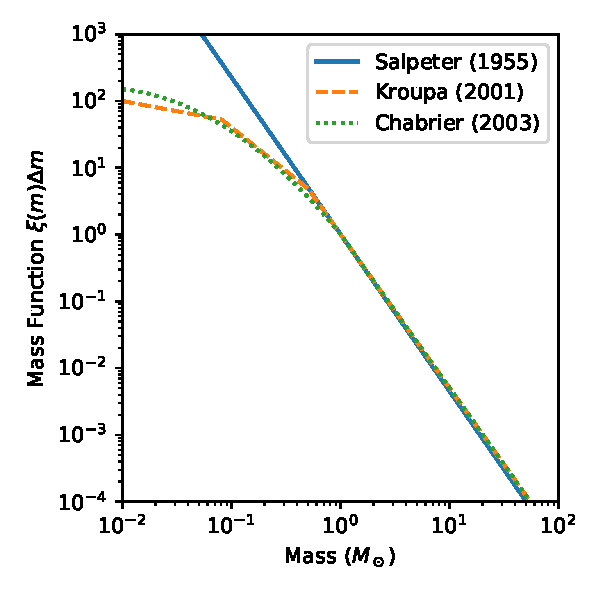
\includegraphics[width=0.5\textwidth]{graphics/star_formation/imf}
    \caption{Comparison of \acp{imf} by \citet{salpeter55}, \citet{kroupa01}, and \citet{chabrier03} normalized to $m=1\,M_\odot$.}
    \label{fig:star_formation:imf}
\end{figure}
Figure~\ref{fig:star_formation:imf} shows the \ac{imf} derived by three different researchers. The first \ac{imf} was published by \citet{salpeter55}. More detailed observations led to revisions of the \ac{imf} by \citet{kroupa01} and \citet{chabrier03}. 
For stars heavier than $1\,M_\odot$, all \acp{imf} agree with each other. At low masses, however, the \ac{imf} by \citet{salpeter55} significantly overestimates the abundance of stars compared to the predictions by \citet{kroupa01} and \citet{chabrier03}. Today, the latter two \acp{imf} are generally used for \ac{gce} models.


\section{The First Stars}\label{sec:star_formation:first_stars}

We have seen above that temperature and cooling play an essential role in star formation. The temperature of a molecular cloud is proportional to the Jeans mass, see equation~\eqref{eqn:star_formation:jeans_mass_derivation}. This leads to two issues: (1) The universe at the beginning was hotter, thus more mass is required for a molecular cloud to undergo gravitational collapse. (2) The main cooling processes of molecular clouds is to radiate heat away to not fall too early into hydrostatic equilibrium. This requires molecules and dust to be present. In the early universe the metallicity was however practically zero, thus this cooling process, except the dissociation of H$_2$ molecules, cannot take place. As a result only very massive, metal-free stars are expected to form in the beginning. 

These predicted, very massive stars with very low metallicity are called population III stars. Metal poor stars with $10^{-4}\,Z_\odot < Z < 10^{-5}\,Z_\odot$, which can mostly be found in old globular clusters, are called population II stars. All more metal-rich stars, mostly found in the galactic disk, are population I stars, e.g., the Sun.

Massive stars, as we will see in detail later on, have a much shorter lifespan than low-mass stars and will thus quickly enrich the early universe with freshly nucleosynthesized products, i.e., metals. Thus, second and later generation will start off with some metallicity. Possible nuclear reactions thus change and get more diverse. To study these earliest stars and nuclosynthesis events, spectroscopic observations of ultra metal-poor stars are an important part. 



\section{Reading}

For the curious reader, Anna Frebel wrote an excellent book titled ``Searching for the Oldest Stars'' \citep{frebel15}. The book is available via the Brandeis Library online.

For the discussion section we will focus on astronomical observations of Reticulum II, an ultrafaint dwarf galaxy that orbits the Milky Way. Please read \citet{croswell21}, a news feature article in the proceedings of the national academy of sciences. This article should give you a very brief and interesting overview of the field of the first stars, \ac{rproc} nuclei, and why they are important for understanding element formation in the universe. Furthermore, this brief article is written as a summary of recent events and discoveries.
Second, please read the paper by \citet{ji16} on the original observations of r-process enhanced stars in Reticulum II. This is the main article that we will discuss in class. The following bullet points should serve as guidance on reading these two manuscripts.
\begin{itemize}
    \item What are r-process nuclides and why are they important in this context?
    \item What are ultrafaint dwarf galaxies? Why are they so interesting when studying the oldest stars? What population of stars do these galaxies contain? What is special about Reticulum II?
    \item Why were neutron star mergers thought to be the main contributor to \ac{rproc} nuclei today, but not in the early universe? Has our thinking changed due to the work by \citet{ji16}? Has our thinking since then changed again?
    \item What is the difference between neutron-capture elements and non-neutron-capture elements? Why is this important in this context?
    \item Why do \citet{ji16} argue that all \ac{rproc} elements in Reticulum II were made by one single event?
    \item What is the neutron star merger to \ac{sn} rate ratio in the Milky Way? What factor do you think play into the determination of the rates?
    \item What alternative scenarios could explain the observations of \citet{ji16} aside from neutron star mergers?
\end{itemize}